\section{Planning}
This section attempts to explain how we planned the course of the project, including what
milestones we set out to reach and what planning methods and artifacts were used to
accomplish this.

After having agreed on a set of project requirements, deadlines, and objectives in
collaboration with the students from Singapore, we needed to plan how to meet those
objectives within the project deadline. As such, we began planning what work needed
to be done and what activities we expected to do in the project.

During the planning process and the associated discussion, it became clear to us that,
in order to make a realistic plan for the project, we needed a more in-depth understanding
of the work and activities lying ahead. 

\label{sec:EmpiriPlanning}
\subsection{Identifying work activities}
After having agreed on a set of project requirements, deadlines and objectives in collaboration with the students from Singapore, we needed to plan how to meet those objectives within the project deadline. As such we began planning what work needed to be done and what activities we expected to do in the project.
During the planning process and the associated discussion it became clear to us, that in order to make a realistic plan for the project, we needed a more in-depth understanding of the work and activities lying ahead. In order to see “the big picture”, we decided to use an approach from KILDEREF known as a work breakdown structure. The work breakdown structure is organized in a hierarchical tree structure, where each new level in the tree is created by dividing a task into subtasks as shown on FIGURE X.X.
 
The division of tasks into smaller components is an iterative process, which stops when the resulting tasks are small enough to be considered a suitable assignment for one man or, more subjectively, when it simply does not make sense to divide it any further.
The use of a work breakdown structure did require several long discussions among the team members regarding the identification of the work. Our use of the work breakdown structure was especially prone to discussion as the problem domain was rather new for us and it was difficult to conclude on what needed to be done, since we had no experience to draw on.
Our complete work breakdown structure can be found in APPENDIXREF
Til analyse-tabere:
Konklusionen som jeg prøver at lægge lidt op til er at vi skulle have brugt product breakdown structure i stedet. Se side 119 i bogen.
Et product breakdown structure sørger for at fokus holdes på HVAD der skal opnås, fremfor HVORDAN det skal opnås og det er specielt velegnet til nye arbejdsområder, hvor det kan være svært at se hvilket arbejde der er nødvendigt, men nemmere at identificere de produkter det skal ende ud i.

\subsection{Identifying activity dependencies}
Having identified the various activities needed to be done, we now tried to make a plan, again, on how to reach the milestones in the project. This time around, we noticed that certain activities had dependencies between them e.g. the \textbf{EXAMPLE1} needed to be done before the \textbf{EXAMPLE2}.
We found it important to gain a firm understanding of the dependencies between our work activities, since we believed this would strengthen our ability to make a realistic plan. As such, we postponed the planning, and instead we strived to strengthen our understanding of the aforementioned dependencies. We decided to use a dependency diagram for this, more precisely a network diagram using the activity on-node format.
In this version of the network diagram, each box represents an activity with dependencies represented as arrows between them. The method uses the concepts of earliest start/finish times (EST/EFT) and latest start/finish times (LST/LFT) in addition to the activity’s own estimated duration.

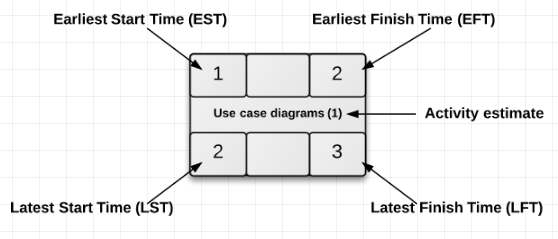
\includegraphics[scale=0.5]{./Empiri/Planning/img/networkdiagramnotation.png}
 
The EST/EFT can be found by a forward pass through the diagram, while the LST/LFTs can be found by a following backward pass.
These numbers introduce the concept of a critical path, which consists of those activities that, if delayed, would delay the whole project (in other words those that must keep the deadline). It also gives a clear presentation of the total slack (how much an activity can be postponed), free slack (how much an activity can be postponed without affecting following activities), and head slack (how much an activity can be postponed without delaying the whole project deadline) for each activity.
Our network diagram can be found in appendix \textbf{insert reference here}.
\subsection{Project planning}
With an overview of our activities’ dependencies and a clear understanding of our
critical path and activity slack, we were ready to plan the project and establish
deadlines.

When making our actual activity plan for the project, we chose to use a planning
tool called a Gantt chart (or Gantt diagram). This chart shows the
activities on one axis with time on the other, which gives an immediate visual
overview of the chronological order of activities (ours can be seen in Appendix
\ref{app:gantt}).

Since we had valuable knowledge about the dependencies of activities (from the
dependency diagram), we chose a variant of the Gantt chart, which also shows these.